## Programas modulares

Revisemos dos ejercicios de la sección de funciones:

\bgnenviron{footnotesize}

\bgnblocknormal
\flushleft{}\vspace{-2ex} Dado un triángulo de lados $a$, $b$ y $c$, escribe una función que calcule su \alert{<2->}{semiperímetro}. Este
valor corresponde a la mitad del perímetro.
\trmblocknormal

\bgnblocknormal
\flushleft{}\vspace{-2ex} La \textsc{fórmula de Herón} nos permite calcular el área de un triángulo sólo usando
el largo de sus tres lados ($a$, $b$ y $c$).
La fórmula es: $$ area = \sqrt{s (s-a) (s-b) (s-c)} $$ donde $s$ es el \alert{<2->}{semiperímetro}.
Escriba una función para calcular el área de un triángulo usando esta fórmula.
\trmblocknormal

\pause

\bgnblockdanger
El primero pedía calcular algo que el segundo necesitaba como insumo para su propio cálculo.
\trmblockdanger

\trmenviron{footnotesize}

## Programas modulares

\simpleTitle{Estrategia de resolución}

- Una de las cosas más importantes es comprender el problema que se debe resolver.
    - Una forma de hacerlo es resolver a mano algunos casos, con datos específicos, para entender a cabalidad todo el problema.

\pause

- Siempre es útil desmenuzar el problema completo en pequeños subproblemas y resolverlos independientemente. 
    - Lo que se debe desarrollar es la habilidad de identificar los subproblemas.

\pause

- Este método se conoce como:

\bgnblockdefinition
\centering  \textbf{Dividir para Reinar}.
\trmblockdefinition

## Programas modulares: Dividir para reinar

- Lo que se debe desarrollar es la habilidad de identificar los subproblemas  que componen el problema original.
    - Para calcular un área, había que calcular previamente un semiperímetro (algo que ya nos pidieron antes).
- Una vez completada la resolución de aquellos subproblemas, podemos armar la solución definitiva.
    - Desde lo más simple, hasta lo más complejo.

- Es más cómodo y eficiente resolver varios problemas pequeños, que uno solo pero mucho más grande.
- Hay que saber cuándo dejar de subdividir.


## Programas modulares {.fragile}

\simpleTitle{Solución del cálculo de la ``Fórmula de Herón'':}

- Primero escribimos la función para calcular el semiperímetro:

\begin{lstlisting}[style=frame02]
# calcSemiperimetro: num num num -> float
# Calcula el semiperímetro de un triángulo, dados sus tres lados.
# Ejemplo: calcSemiperimetro(3, 4, 5) retorna 6
def calcSemiperimetro(a, b, c):
    return (a + b + c) / 2.0 (*@ \tikzmark{mrkfloatdiv} @*)
# Test
assert calcSemiperimetro(3, 4, 5) == 6
assert calcSemiperimetro(13, 10, 8) == 15.5
\end{lstlisting}

\pause

  \drawTikZComment{mrkfloatdiv}{OJO: la división debe ser \nzinlinecode{float}}

## Programas modulares {.fragile}

\simpleTitle{Solución del cálculo de la ``Fórmula de Herón'':}

- Y después, la función para calcular el área:

\begin{lstlisting}[style=frame02]
# areaTriangulo: num num num -> float
# Calcula el área de un triángulo, dados sus tres lados,
# usando la fórmula de Herón.
# Ejemplo: areaTriangulo(3, 4, 5) retorna 6
def areaTriangulo(a, b, c):
    semip = calcSemiperimetro(a, b, c) (*@\tikzmark{mrksubproc}@*)
    return (semip * (semip - a) * (semip - b) * (semip - c))**0.5
# Test
assert areaTriangulo(3, 4, 5) == 6.0
assert areaTriangulo(13, 10, 8) == 39.98046397929869
assert areaTriangulo(12, 14, 3) == 14.43736471798091
\end{lstlisting}

\pause

  \drawTikZComment[above right=2mm and 8mm of mrksubproc, text width = 40mm]{mrksubproc}{Acá usamos la función \nzinlinecode{calcSemiperimetro}.}

## Programas modulares {.fragile}

\simpleTitle{Solución del cálculo de la ``Fórmula de Herón'':}

- Hay una discusión que es necesaria en este caso:

\bgnblocknormal
¿Es tan común calcular el semiperímetro de un triángulo?  \newline
¿No será más común calcular su perímetro?
\trmblocknormal

\pause

- Efectivamente, es más común calcular sólo el perímetro.

\bgnblockidea
\strongText{Ejercicio propuesto}: Vuelve a programar la fórmula de Herón, pero esta vez usando la función
que calcula el \structure{perímetro} de un triángulo.
\trmblockidea

## Programar módulos en Python {.fragile}

- Hasta ahora, hemos estado programando dentro de IDLE.
    - Es fácil hacer pruebas rápidas de código.
    - Se puede definir funciones y después usarlas.

- Sin embargo:
    - No es tan fácil volver a reutilizar código.

\pause

\bgnblockidea
Nos convendría guardar nuestro código en algún archivo que después podamos volver a utilizar, incluso en
otro computador.
\trmblockidea

\pause

\bgnblockdefinition
\bld{Archivos .py:} Son archivos de texto en los cuales se escribe código Python que puede ser usado
cuando queramos.
\trmblockdefinition

## Programar módulos en Python {.fragile}

- Desde ahora en adelante, para poder reutilizar código haremos lo siguiente:
    - Escribiremos nuestros programas en \bld{módulos}.
    - Cada módulo estará en su respectivo archivo \bld{.py}.

- Implementemos un ejemplo sencillo, para empezar:

\bgnblocknormal
Calculemos el área de un rombo
\trmblocknormal


## Ejemplo: Calcular el área de un rombo

Recordemos cómo se define un rombo\footnote{\tiny{Diagrama bajo licencia Creative Commons, copiada desde http://en.wikipedia.org/wiki/File:Rhombus1.svg}}:

- Es un cuadrilátero (4 lados).
- Es paralelógramo (lados opuestos paralelos).
- Sus cuatro lados tienen la misma longitud.

\vspace{4mm}

\begin{center}
    \begin{figure}
    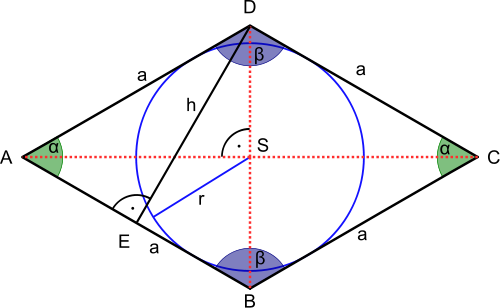
\includegraphics[width=.5\textwidth]{img/rhombus-500px.png}
    \caption{Un rombo}
    \end{figure}
\end{center}


## Ejemplo: Calcular el área de un rombo

Existen varias maneras de representar (definir) un rombo:
\begin{enumerate}
    \footnotesize
    \item Longitud de sus lados (\textbf{a}) y los ángulos interiores ($\alpha$ y $\beta$).
    \item Longitud de sus lados (\textbf{a}) y del radio (\textbf{r}) de la circunferencia inscrita.
    \item Longitud de sus dos diagonales (\textbf{p} y \textbf{q}).
    \item \alert<2->{Las cuatro coordenadas de sus vértices: (\textbf{$ (x_a, y_a), (x_b, y_b), (x_c, y_c), (x_d, y_d)$}).}
\end{enumerate}

\vspace{4mm}
Para cada una de estas definiciones, se tiene una manera de calcular su área:
\begin{enumerate}
    \footnotesize
    \item \parbox{27mm}{(a, $\alpha$, $\beta$)} $ A = a^2 * sen(\alpha) = a^2 * sen(\beta) $
    \item \parbox{27mm}{(a, r)} $ A = 2a * r $
    \item \parbox{27mm}{(p, q)} $ A = \frac{p * q}{2} $
    \item \alert<2->{\parbox{27mm}{Coordenadas} $ A = \left( \frac{\sqrt{(x_c - x_a)^2 + (y_c - y_a)^2} * \sqrt{(x_d - x_b)^2 + (y_d - y_b)^2}}{2} \right) $}
\end{enumerate}

## Ejemplo: Calcular el área de un rombo

\vspace*{-12mm}

\bgncolumns

\column{0.48\textwidth}
\begin{figure}
\begin{tikzflowchart}
  \matrix (e) [matrix of nodes, column sep=5mm, row sep=4mm]%
  {
    \node [startstop] (p1) {INICIO}; \\
    \node [io, text width=34mm] (p2) {Obtener las coordenadas:\\$x_a, y_a, x_b, y_b, x_c, y_c, x_d, y_d$}; \\
    \node [predefproc] (p3) {$ \mathtt{d_{ca}} $ = largoDe(c, a)}; \\
    \node [predefproc] (p4) {$ \mathtt{d_{db}} $ = largoDe(d, b)}; \\
    \node [process] (p5) {$ \mathtt{A = d_{ca} * d_{db} / 2} $}; \\
    \node [io] (p6) {Entregamos \ttt{A}}; \\
    \node [startstop] (p7) {FIN}; \\
  };

  { [start chain]
    \chainin (p1);
    \chainin (p2) [join=by arrow];
    \chainin (p3) [join=by arrow];
    \chainin (p4) [join=by arrow];
    \chainin (p5) [join=by arrow];
    \chainin (p6) [join=by arrow];
    \chainin (p7) [join=by arrow];
  }
\end{tikzflowchart}

\caption{Diagrama del proceso completo.}
\end{figure}

\pause

\column{0.04\textwidth}

\column{0.48\textwidth}

\begin{figure}
\begin{tikzflowchart}

  \matrix (e) [matrix of nodes, column sep=5mm, row sep=4mm]%
  {
    \node [startstop] (p1) {INICIO}; \\
    \node [io, text width=30mm] (p2) {Obtener las coordenadas:\\$x_1, y_1, x_2, y_2$}; \\
    \node [process] (p5) {$ \mathtt{f = (x_2-x_1)^2 + (y_2-y_1)^2} $}; \\
    \node [io] (p6) {Entregamos: $ \mathtt{ \sqrt{f} } $}; \\
    \node [startstop] (p7) {FIN}; \\
  };

  { [start chain]
    \chainin (p1);
    \chainin (p2) [join=by arrow];
    \chainin (p5) [join=by arrow];
    \chainin (p6) [join=by arrow];
    \chainin (p7) [join=by arrow];
  }

  \node[draw, fit=(p1) (p2) (p7), inner sep=1em] (enc) {};
  \node[above=0mm of enc.north, text centered, text width=40mm] {Calcular el largo de un segmento, dados sus dos puntos.};
\end{tikzflowchart}

\caption{Diagrama del subproceso \ttt{largoDe}.}
\end{figure}

\trmcolumns

## Ejemplo: Calcular el área de un rombo {.fragile}

\simpleTitle*{Solución:}

\begin{lstlisting}[basicstyle=\scriptsize\ttfamily,style=frame01]
# largoSegmento: num num num num -> float
# Calcula el largo del segmento entre los dos
# puntos cuyas coordenadas se entregan.
# Ejemplo: largoSegmento(0, -1, 0, 1) retorna 2.0
def largoSegmento(px, py, qx, qy):
    sqrSum = (qx - px)**2 + (qy - py)**2
    return sqrSum**0.5
# Test
assert largoSegmento(4, 0, 0, 3) == 5.0

# areaRombo: num num num num num num num num -> float
# Calcula el área de un rombo, dadas las
# coordenadas de sus cuatro vértices
# Ejemplo: areaRombo(-2, 0, 0, -1, 2, 0, 0, 1) retorna 4.0
def areaRombo(ax, ay, bx, by, cx, cy, dx, dy):
    diagAC = largoSegmento(ax, ay, cx, cy)
    diagBD = largoSegmento(bx, by, dx, dy)
    return diagAC * diagBD / 2.0
# Test
assert areaRombo(-3, 0, 0, -1, 3, 0, 0, 1) == 6.0
\end{lstlisting}
